\documentclass[a4paper]{article}
\usepackage{parskip}

\def\nterm {Spring}
\def\nyear {2025}
\def\ncourse {Natural Language Processing}

\makeatletter
\ifx \nauthor\undefined
  \def\nauthor{Runqiu Ye}
\else
\fi

\author{Notes taken by \nauthor\vspace{5pt}\\
Carnegie Mellon University}
\date{\nterm\ \nyear}

\usepackage{alltt}
\usepackage{amsfonts}
\usepackage{amsmath}
\usepackage{amssymb}
\usepackage{amsthm}
\usepackage{booktabs}
\usepackage{caption}
\usepackage{enumitem}
\usepackage{fancyhdr}
\usepackage{graphicx}
\usepackage{mathdots}
\usepackage{mathtools}
\usepackage{microtype}
\usepackage{multirow}
\usepackage{pdflscape}
\usepackage{pgfplots}
\usepackage{siunitx}
\usepackage{slashed}
\usepackage{tabularx}
\usepackage{tikz}
\usepackage{tkz-euclide}
\usepackage[normalem]{ulem}
\usepackage[all]{xy}
\usepackage{imakeidx}
\usepackage{mathrsfs}
\usepackage[includehead,includefoot,heightrounded,left=1.25in,right=1.25in]{geometry}

\makeindex[intoc, title=Index]
\indexsetup{othercode={\lhead{\emph{Index}}}}

\ifx \nextra \undefined
  \usepackage[pdftex,
    hidelinks,
    pdfauthor={Dexter Chua},
    pdfsubject={\ncourse},
    pdftitle={\ncourse},
  pdfkeywords={Cambridge Mathematics Maths Math \nterm\ \nyear\ \ncourse}]{hyperref}
  \title{\ncourse}
\else
  \usepackage[pdftex,
    hidelinks,
    pdfauthor={Dexter Chua},
    pdfsubject={Cambridge Maths Notes: \ncourse\ (\nextra)},
    pdftitle={\ncourse\ (\nextra)},
  pdfkeywords={Cambridge Mathematics Maths Math \nterm\ \nyear\ \ncourse\ \nextra}]{hyperref}

  \title{\ncourse \\ {\Large \nextra}}
  \renewcommand\printindex{}
\fi

\pgfplotsset{compat=1.12}

\pagestyle{fancyplain}
\ifx \ncoursehead \undefined
\def\ncoursehead{\ncourse}
\fi

\lhead{\emph{\nouppercase{\leftmark}}}
\ifx \nextra \undefined
  \rhead{
    \ifnum\thepage=1
    \else
      \ncoursehead
    \fi}
\else
  \rhead{
    \ifnum\thepage=1
    \else
      \ncoursehead \ (\nextra)
    \fi}
\fi
\usetikzlibrary{arrows.meta}
\usetikzlibrary{decorations.markings}
\usetikzlibrary{decorations.pathmorphing}
\usetikzlibrary{positioning}
\usetikzlibrary{fadings}
\usetikzlibrary{intersections}
\usetikzlibrary{cd}

\newcommand*{\Cdot}{{\raisebox{-0.25ex}{\scalebox{1.5}{$\cdot$}}}}
\newcommand {\pd}[2][ ]{
  \ifx #1 { }
    \frac{\partial}{\partial #2}
  \else
    \frac{\partial^{#1}}{\partial #2^{#1}}
  \fi
}
\ifx \nhtml \undefined
\else
  \renewcommand\printindex{}
  \DisableLigatures[f]{family = *}
  \let\Contentsline\contentsline
  \renewcommand\contentsline[3]{\Contentsline{#1}{#2}{}}
  \renewcommand{\@dotsep}{10000}
  \newlength\currentparindent
  \setlength\currentparindent\parindent

  \newcommand\@minipagerestore{\setlength{\parindent}{\currentparindent}}
  \usepackage[active,tightpage,pdftex]{preview}
  \renewcommand{\PreviewBorder}{0.1cm}

  \newenvironment{stretchpage}%
  {\begin{preview}\begin{minipage}{\hsize}}%
    {\end{minipage}\end{preview}}
  \AtBeginDocument{\begin{stretchpage}}
  \AtEndDocument{\end{stretchpage}}

  \newcommand{\@@newpage}{\end{stretchpage}\begin{stretchpage}}

  \let\@real@section\section
  \renewcommand{\section}{\@@newpage\@real@section}
  \let\@real@subsection\subsection
  \renewcommand{\subsection}{\@ifstar{\@real@subsection*}{\@@newpage\@real@subsection}}
\fi
\ifx \ntrim \undefined
\else
  \usepackage{geometry}
  \geometry{
    papersize={379pt, 699pt},
    textwidth=345pt,
    textheight=596pt,
    left=17pt,
    top=54pt,
    right=17pt
  }
\fi

\ifx \nisofficial \undefined
\let\@real@maketitle\maketitle
\renewcommand{\maketitle}{\@real@maketitle}
\else
\fi

% Theorems
\theoremstyle{definition}
\newtheorem*{aim}{Aim}
\newtheorem*{axiom}{Axiom}
\newtheorem*{claim}{Claim}
\newtheorem*{cor}{Corollary}
\newtheorem*{conjecture}{Conjecture}
\newtheorem*{defi}{Definition}
\newtheorem*{eg}{Example}
\newtheorem*{ex}{Exercise}
\newtheorem*{fact}{Fact}
\newtheorem*{law}{Law}
\newtheorem*{lemma}{Lemma}
\newtheorem*{notation}{Notation}
\newtheorem*{prop}{Proposition}
\newtheorem*{question}{Question}
\newtheorem*{rrule}{Rule}
\newtheorem*{thm}{Theorem}
\newtheorem*{assumption}{Assumption}
\newtheorem*{algorithm}{Algorithm}

\newtheorem*{remark}{Remark}
\newtheorem*{warning}{Warning}
\newtheorem*{exercise}{Exercise}

\newtheorem{nthm}{Theorem}[section]
\newtheorem{nlemma}[nthm]{Lemma}
\newtheorem{nprop}[nthm]{Proposition}
\newtheorem{ncor}[nthm]{Corollary}


\renewcommand{\labelitemi}{--}
\renewcommand{\labelitemii}{$\circ$}
% \renewcommand{\labelenumi}{(\roman{*})}

\let\stdsection\section
\renewcommand\section{\newpage\stdsection}

\newcommand\qedsym{\hfill\ensuremath{\square}}
% Strike through
\def\st{\bgroup \ULdepth=-.55ex \ULset}


%%%%%%%%%%%%%%%%%%%%%%%%%
%%%%% Maths Symbols %%%%%
%%%%%%%%%%%%%%%%%%%%%%%%%
\renewcommand{\epsilon}{\varepsilon}
\renewcommand{\phi}{\varphi}

\renewcommand{\bar}[1]{\overline{#1}}
\renewcommand{\tilde}[1]{\widetilde{#1}}
\renewcommand{\hat}[1]{\widehat{#1}}

% training examples
\newcommand{\xii}{x^{(i)}}
\newcommand{\yii}{y^{(i)}}

% machine learning 
\DeclareMathOperator{\VC}{VC}
\DeclareMathOperator{\err}{err}
\DeclareMathOperator{\bits}{bits}
\DeclareMathOperator{\reg}{reg}
\DeclareMathOperator{\risk}{risk}

% Matrix groups
\newcommand{\GL}{\mathrm{GL}}
\newcommand{\Or}{\mathrm{O}}
\newcommand{\PGL}{\mathrm{PGL}}
\newcommand{\PSL}{\mathrm{PSL}}
\newcommand{\PSO}{\mathrm{PSO}}
\newcommand{\PSU}{\mathrm{PSU}}
\newcommand{\SL}{\mathrm{SL}}
\newcommand{\SO}{\mathrm{SO}}
\newcommand{\Spin}{\mathrm{Spin}}
\newcommand{\Sp}{\mathrm{Sp}}
\newcommand{\SU}{\mathrm{SU}}
\newcommand{\U}{\mathrm{U}}
\newcommand{\Mat}{\mathrm{Mat}}

% Matrix algebras
\newcommand{\gl}{\mathfrak{gl}}
\newcommand{\ort}{\mathfrak{o}}
\newcommand{\so}{\mathfrak{so}}
\newcommand{\su}{\mathfrak{su}}
\newcommand{\uu}{\mathfrak{u}}
\renewcommand{\sl}{\mathfrak{sl}}

% Special sets
\newcommand{\C}{\mathbb{C}}
\newcommand{\CP}{\mathbb{CP}}
\newcommand{\GG}{\mathbb{G}}
\newcommand{\N}{\mathbb{N}}
\newcommand{\Q}{\mathbb{Q}}
\newcommand{\R}{\mathbb{R}}
\newcommand{\RP}{\mathbb{RP}}
\newcommand{\T}{\mathbb{T}}
\newcommand{\Z}{\mathbb{Z}}
% \renewcommand{\H}{\mathbb{H}}

% Brackets
\newcommand{\floor}[1]{\left\lfloor #1 \right\rfloor}
\newcommand{\ceil}[1]{\left\lceil #1 \right\rceil}
\newcommand{\abs}[1]{\left\lvert #1\right\rvert}
\newcommand{\bket}[1]{\left\lvert #1\right\rangle}
\newcommand{\brak}[1]{\left\langle #1 \right\rvert}
\newcommand{\braket}[2]{\left\langle #1, #2 \right\rangle}
\newcommand{\bra}{\langle}
\newcommand{\ket}{\rangle}
\newcommand{\norm}[1]{\left\lVert #1\right\rVert}
\newcommand{\normalorder}[1]{\mathop{:}\nolimits\!#1\!\mathop{:}\nolimits}
\renewcommand{\vec}[1]{\boldsymbol{\mathbf{#1}}}
\DeclareMathOperator{\curl}{curl}
\DeclareMathOperator{\diverge}{div}
\DeclareMathOperator{\dist}{dist}

% not-math
\newcommand{\bolds}[1]{{\bfseries #1}}
\newcommand{\cat}[1]{\mathsf{#1}}
\newcommand{\ph}{\,\cdot\,}
\newcommand{\term}[1]{\emph{#1}\index{#1}}
\newcommand{\phantomeq}{\hphantom{{}={}}}

% Probability
\newcommand{\ind}{\mathbf{1}}
\newcommand{\convAS}{\overset{\mathrm{as}}{\longrightarrow}}
\newcommand{\convProb}{\overset{\mathrm{P}}{\longrightarrow}}
\newcommand{\convDist}{\rightsquigarrow}
\newcommand{\convQM}{\overset{\mathrm{qm}}{\longrightarrow}}
\DeclareMathOperator{\Bernoulli}{Bernoulli}
\DeclareMathOperator{\betaD}{beta}
\DeclareMathOperator{\bias}{bias}
\DeclareMathOperator{\binomial}{binomial}
\DeclareMathOperator{\corr}{corr}
\DeclareMathOperator{\cov}{cov}
\DeclareMathOperator{\gammaD}{gamma}
\DeclareMathOperator{\mse}{MSE}
\DeclareMathOperator{\multinomial}{multinomial}
\DeclareMathOperator{\Poisson}{Poisson}
\DeclareMathOperator{\var}{var}
\newcommand{\E}{\mathbb{E}}
\renewcommand{\Pr}{\mathbb{P}}
\newcommand{\KLD}[2]{\mathrm{KL}(#1 \; \Vert \; #2)}
\newcommand{\const}{\mathrm{const}}
\DeclareMathOperator{\KL}{KL}

% Algebra
\DeclareMathOperator{\adj}{adj}
\DeclareMathOperator{\Ann}{Ann}
\DeclareMathOperator{\Aut}{Aut}
\DeclareMathOperator{\Char}{char}
\DeclareMathOperator{\disc}{disc}
\DeclareMathOperator{\dom}{dom}
\DeclareMathOperator{\fix}{fix}
\DeclareMathOperator{\Hom}{Hom}
\DeclareMathOperator{\id}{id}
\DeclareMathOperator{\image}{image}
\DeclareMathOperator{\im}{im}
\DeclareMathOperator{\tr}{tr}
\DeclareMathOperator{\Tr}{Tr}
\newcommand{\Bilin}{\mathrm{Bilin}}
\newcommand{\Frob}{\mathrm{Frob}}

% Others
\newcommand\ad{\mathrm{ad}}
\newcommand\Art{\mathrm{Art}}
\newcommand{\B}{\mathcal{B}}
\newcommand{\cU}{\mathcal{U}}
\newcommand{\Der}{\mathrm{Der}}
\newcommand{\D}{\mathrm{D}}
\newcommand{\dR}{\mathrm{dR}}
\newcommand{\exterior}{\mathchoice{{\textstyle\bigwedge}}{{\bigwedge}}{{\textstyle\wedge}}{{\scriptstyle\wedge}}}
\newcommand{\F}{\mathbb{F}}
\newcommand{\G}{\mathcal{G}}
\newcommand{\Gr}{\mathrm{Gr}}
\newcommand{\haut}{\mathrm{ht}}
\newcommand{\Hol}{\mathrm{Hol}}
\newcommand{\hol}{\mathfrak{hol}}
\newcommand{\Id}{\mathrm{Id}}
\newcommand{\lie}[1]{\mathfrak{#1}}
\newcommand{\op}{\mathrm{op}}
\newcommand{\Oc}{\mathcal{O}}
\newcommand{\pr}{\mathrm{pr}}
\newcommand{\Ps}{\mathcal{P}}
\newcommand{\pt}{\mathrm{pt}}
\newcommand{\qeq}{\mathrel{``{=}"}}
\newcommand{\Rs}{\mathcal{R}}
\newcommand{\Vect}{\mathrm{Vect}}
\newcommand{\wsto}{\stackrel{\mathrm{w}^*}{\to}}
\newcommand{\wt}{\mathrm{wt}}
\newcommand{\wto}{\stackrel{\mathrm{w}}{\to}}
\renewcommand{\d}{\mathrm{d}}


\let\Im\relax
\let\Re\relax

\DeclareMathOperator{\softmax}{softmax}
\DeclareMathOperator*{\argmax}{argmax}
\DeclareMathOperator*{\argmin}{argmin}
\DeclareMathOperator{\area}{area}
\DeclareMathOperator{\card}{card}
\DeclareMathOperator{\ccl}{ccl}
\DeclareMathOperator{\ch}{ch}
\DeclareMathOperator{\cl}{cl}
\DeclareMathOperator{\cls}{\overline{\mathrm{span}}}
\DeclareMathOperator{\coker}{coker}
\DeclareMathOperator{\conv}{conv}
\DeclareMathOperator{\cosec}{cosec}
\DeclareMathOperator{\cosech}{cosech}
\DeclareMathOperator{\covol}{covol}
\DeclareMathOperator{\diag}{diag}
\DeclareMathOperator{\diam}{diam}
\DeclareMathOperator{\Diff}{Diff}
\DeclareMathOperator{\End}{End}
\DeclareMathOperator{\energy}{energy}
\DeclareMathOperator{\erfc}{erfc}
\DeclareMathOperator{\erf}{erf}
\DeclareMathOperator*{\esssup}{ess\,sup}
\DeclareMathOperator{\Ext}{Ext}
\DeclareMathOperator{\fst}{fst}
\DeclareMathOperator{\Fit}{Fit}
\DeclareMathOperator{\Frac}{Frac}
\DeclareMathOperator{\Gal}{Gal}
\DeclareMathOperator{\gr}{gr}
\DeclareMathOperator{\hcf}{hcf}
\DeclareMathOperator{\Im}{Im}
\DeclareMathOperator{\Ind}{Ind}
\DeclareMathOperator{\Int}{Int}
\DeclareMathOperator{\Isom}{Isom}
\DeclareMathOperator{\lcm}{lcm}
\DeclareMathOperator{\length}{length}
\DeclareMathOperator{\Lie}{Lie}
\DeclareMathOperator{\like}{like}
\DeclareMathOperator{\Lk}{Lk}
\DeclareMathOperator{\Maps}{Maps}
\DeclareMathOperator{\orb}{orb}
\DeclareMathOperator{\ord}{ord}
\DeclareMathOperator{\otp}{otp}
\DeclareMathOperator{\poly}{poly}
\DeclareMathOperator{\rank}{rank}
\DeclareMathOperator{\rel}{rel}
\DeclareMathOperator{\Rad}{Rad}
\DeclareMathOperator{\Re}{Re}
\DeclareMathOperator*{\res}{res}
\DeclareMathOperator{\Res}{Res}
\DeclareMathOperator{\Ric}{Ric}
\DeclareMathOperator{\rk}{rk}
\DeclareMathOperator{\Rees}{Rees}
\DeclareMathOperator{\Root}{Root}
\DeclareMathOperator{\sech}{sech}
\DeclareMathOperator{\sign}{sign}
\DeclareMathOperator{\snd}{snd}
\DeclareMathOperator{\Spec}{Spec}
\DeclareMathOperator{\spn}{span}
\DeclareMathOperator{\stab}{stab}
\DeclareMathOperator{\St}{St}
\DeclareMathOperator{\supp}{supp}
\DeclareMathOperator{\Syl}{Syl}
\DeclareMathOperator{\Sym}{Sym}
\DeclareMathOperator{\vol}{vol}

% mathbf lowercase
\newcommand{\av}{\vec{a}}
\newcommand{\bv}{\vec{b}}
\newcommand{\cv}{\vec{c}}
\newcommand{\dv}{\vec{d}}
\newcommand{\ev}{\vec{e}}
\newcommand{\fv}{\vec{f}}
\newcommand{\gv}{\vec{g}}
\newcommand{\hv}{\vec{h}}
\newcommand{\iv}{\vec{i}}
\newcommand{\jv}{\vec{j}}
\newcommand{\kv}{\vec{k}}
\newcommand{\lv}{\vec{l}}
\newcommand{\mv}{\vec{m}}
\newcommand{\nv}{\vec{n}}
\newcommand{\ov}{\vec{o}}
\newcommand{\pv}{\vec{p}}
\newcommand{\qv}{\vec{q}}
\newcommand{\rv}{\vec{r}}
\newcommand{\sv}{\vec{s}}
\newcommand{\tv}{\vec{t}}
\newcommand{\uv}{\vec{u}}
\newcommand{\vv}{\vec{v}}
\newcommand{\wv}{\vec{w}}
\newcommand{\xv}{\vec{x}}
\newcommand{\yv}{\vec{y}}
\newcommand{\zv}{\vec{z}}

% mathbf uppercase
\newcommand{\Av}{\vec{A}}
\newcommand{\Bv}{\vec{B}}
\newcommand{\Cv}{\vec{C}}
\newcommand{\Dv}{\vec{D}}
\newcommand{\Ev}{\vec{E}}
\newcommand{\Fv}{\vec{F}}
\newcommand{\Gv}{\vec{G}}
\newcommand{\Hv}{\vec{H}}
\newcommand{\Iv}{\vec{I}}
\newcommand{\Jv}{\vec{J}}
\newcommand{\Kv}{\vec{K}}
\newcommand{\Lv}{\vec{L}}
\newcommand{\Mv}{\vec{M}}
\newcommand{\Nv}{\vec{N}}
\newcommand{\Ov}{\vec{O}}
\newcommand{\Pv}{\vec{P}}
\newcommand{\Qv}{\vec{Q}}
\newcommand{\Rv}{\vec{R}}
\newcommand{\Sv}{\vec{S}}
\newcommand{\Tv}{\vec{T}}
\newcommand{\Uv}{\vec{U}}
\newcommand{\Vv}{\vec{V}}
\newcommand{\Wv}{\vec{W}}
\newcommand{\Xv}{\vec{X}}
\newcommand{\Yv}{\vec{Y}}
\newcommand{\Zv}{\vec{Z}}

% mathscr 
\newcommand{\hscr}{\mathscr{H}}

% mathcal
\newcommand{\acal}{\mathcal{A}}
\newcommand{\ecal}{\mathcal{E}}
\newcommand{\fcal}{\mathcal{F}}
\newcommand{\hcal}{\mathcal{H}}
\renewcommand{\L}{\mathcal{L}}
\newcommand{\ncal}{\mathcal{N}}
\renewcommand{\P}{\mathcal{P}}
\renewcommand{\Q}{\mathcal{Q}}
\newcommand{\rcal}{\mathcal{R}}

\pgfarrowsdeclarecombine{twolatex'}{twolatex'}{latex'}{latex'}{latex'}{latex'}
\tikzset{->/.style = {decoration={markings,
                                  mark=at position 1 with {\arrow[scale=2]{latex'}}},
                      postaction={decorate}}}
\tikzset{<-/.style = {decoration={markings,
                                  mark=at position 0 with {\arrowreversed[scale=2]{latex'}}},
                      postaction={decorate}}}
\tikzset{<->/.style = {decoration={markings,
                                   mark=at position 0 with {\arrowreversed[scale=2]{latex'}},
                                   mark=at position 1 with {\arrow[scale=2]{latex'}}},
                       postaction={decorate}}}
\tikzset{->-/.style = {decoration={markings,
                                   mark=at position #1 with {\arrow[scale=2]{latex'}}},
                       postaction={decorate}}}
\tikzset{-<-/.style = {decoration={markings,
                                   mark=at position #1 with {\arrowreversed[scale=2]{latex'}}},
                       postaction={decorate}}}
\tikzset{->>/.style = {decoration={markings,
                                  mark=at position 1 with {\arrow[scale=2]{latex'}}},
                      postaction={decorate}}}
\tikzset{<<-/.style = {decoration={markings,
                                  mark=at position 0 with {\arrowreversed[scale=2]{twolatex'}}},
                      postaction={decorate}}}
\tikzset{<<->>/.style = {decoration={markings,
                                   mark=at position 0 with {\arrowreversed[scale=2]{twolatex'}},
                                   mark=at position 1 with {\arrow[scale=2]{twolatex'}}},
                       postaction={decorate}}}
\tikzset{->>-/.style = {decoration={markings,
                                   mark=at position #1 with {\arrow[scale=2]{twolatex'}}},
                       postaction={decorate}}}
\tikzset{-<<-/.style = {decoration={markings,
                                   mark=at position #1 with {\arrowreversed[scale=2]{twolatex'}}},
                       postaction={decorate}}}

\tikzset{circ/.style = {fill, circle, inner sep = 0, minimum size = 3}}
\tikzset{scirc/.style = {fill, circle, inner sep = 0, minimum size = 1.5}}
\tikzset{mstate/.style={circle, draw, blue, text=black, minimum width=0.7cm}}

\tikzset{eqpic/.style={baseline={([yshift=-.5ex]current bounding box.center)}}}
\tikzset{commutative diagrams/.cd,cdmap/.style={/tikz/column 1/.append style={anchor=base east},/tikz/column 2/.append style={anchor=base west},row sep=tiny}}

\definecolor{mblue}{rgb}{0.2, 0.3, 0.8}
\definecolor{morange}{rgb}{1, 0.5, 0}
\definecolor{mgreen}{rgb}{0.1, 0.4, 0.2}
\definecolor{mred}{rgb}{0.5, 0, 0}

\def\drawcirculararc(#1,#2)(#3,#4)(#5,#6){%
    \pgfmathsetmacro\cA{(#1*#1+#2*#2-#3*#3-#4*#4)/2}%
    \pgfmathsetmacro\cB{(#1*#1+#2*#2-#5*#5-#6*#6)/2}%
    \pgfmathsetmacro\cy{(\cB*(#1-#3)-\cA*(#1-#5))/%
                        ((#2-#6)*(#1-#3)-(#2-#4)*(#1-#5))}%
    \pgfmathsetmacro\cx{(\cA-\cy*(#2-#4))/(#1-#3)}%
    \pgfmathsetmacro\cr{sqrt((#1-\cx)*(#1-\cx)+(#2-\cy)*(#2-\cy))}%
    \pgfmathsetmacro\cA{atan2(#2-\cy,#1-\cx)}%
    \pgfmathsetmacro\cB{atan2(#6-\cy,#5-\cx)}%
    \pgfmathparse{\cB<\cA}%
    \ifnum\pgfmathresult=1
        \pgfmathsetmacro\cB{\cB+360}%
    \fi
    \draw (#1,#2) arc (\cA:\cB:\cr);%
}
\newcommand\getCoord[3]{\newdimen{#1}\newdimen{#2}\pgfextractx{#1}{\pgfpointanchor{#3}{center}}\pgfextracty{#2}{\pgfpointanchor{#3}{center}}}

\newcommand\qedshift{\vspace{-17pt}}
\newcommand\fakeqed{\pushQED{\qed}\qedhere}

\def\Xint#1{\mathchoice
   {\XXint\displaystyle\textstyle{#1}}%
   {\XXint\textstyle\scriptstyle{#1}}%
   {\XXint\scriptstyle\scriptscriptstyle{#1}}%
   {\XXint\scriptscriptstyle\scriptscriptstyle{#1}}%
   \!\int}
\def\XXint#1#2#3{{\setbox0=\hbox{$#1{#2#3}{\int}$}
     \vcenter{\hbox{$#2#3$}}\kern-.5\wd0}}
\def\ddashint{\Xint=}
\def\dashint{\Xint-}

\newcommand\separator{{\centering\rule{2cm}{0.2pt}\vspace{2pt}\par}}

\newenvironment{own}{\color{gray!70!black}}{}

\newcommand\makecenter[1]{\raisebox{-0.5\height}{#1}}

\mathchardef\mdash="2D

\newenvironment{significant}{\begin{center}\begin{minipage}{0.9\textwidth}\centering\em}{\end{minipage}\end{center}}
\DeclareRobustCommand{\rvdots}{%
  \vbox{
    \baselineskip4\p@\lineskiplimit\z@
    \kern-\p@
    \hbox{.}\hbox{.}\hbox{.}
  }}
\DeclareRobustCommand\tph[3]{{\texorpdfstring{#1}{#2}}}
\makeatother


\begin{document}
\maketitle

\tableofcontents

\section{Introduction}

Below is a list of topics that will be covered in this note. 
The topics include fundamental theoretical knowledge in 
language processing and language modeling in the first 
few sections, as well as frontier research results
in later sections.

\begin{enumerate}
  \item Language modeling fundamentals 
  \begin{enumerate}
    \item Representing words 
    \item Language modeling 
    \item Sequence modeling architectures
  \end{enumerate}

  \item Training and inference models
  \begin{enumerate}
    \item Decoding and Generation Algorithms
    \item In-context learning
    \item Pre-training
    \item Fine-tuning
    \item Reinforcement Learning
  \end{enumerate}

  \item Evaluation and Experimental Design
  \begin{enumerate}
    \item Evaluating Language Generators
    \item Experimental Design
    \item Human Annotation
    \item Debugging/Interpretation Techniques
  \end{enumerate}

  \item Advanced Algorithms and Architectures 
  \begin{enumerate}
    \item Advanced Pretraining, Post-Training, and Inference
    \item Retrieval and Retrieval-augmented Generation
    \item Long Sequence Models
    \item Distillation and Quantization
    \item Ensembling and Mixture of Experts
  \end{enumerate}

  \item NLP Applications and Society
  \begin{enumerate}
    \item Complex Reasoning Tasks
    \item Language Agents
    \item Multimodal NLP
    \item Multilingual NLP
    \item Bias and Fairness
  \end{enumerate}
\end{enumerate}

\section{Language modeling fundamentals}

\subsection{Neural networks and auto differentiation}
This process calculates the gradient of the loss with 
respect to different parameters. Use computational graph 
and chain rule to compute back propogation efficiently, 
and implmented in PyTorch. With the calculated gradient, 
we can use Stochastic Gradient Descent (SGD) to update 
the model parameters. 
Other than PyTorch, TensorFlow and JAX are also popular 
neural network frameworks with different advantages.

\subsection{language and sequence modeling} 

In language modeling, other than binary or multi-class 
classification, sometimes there are exponential/infinitely
many labels. This is called \textbf{structured prediction}. 
For example, assgining a part-of-speech tag for each word in the 
sentence. It is easy to note that in this case the number 
of labels grows exponentially with respect to the length 
of the sequence.
There are also distinctions between \textbf{uncondictioned 
prediction} and \textbf{conditioned prediction}, which predict 
the distribution of $P(X)$ and $P(Y \mid X)$, respectively.

A language model is a probability distribution over all 
sequences. It can be used to \textbf{score} sequences
and \textbf{generate} sequences. For example, in 
conditional generation, we condition on an input text and 
tries to continue it 
\[
\hat{x}_{t + 1: T} \sim p(X_{t+1: T} \mid x_{1 : t}).
\]
For another example, it can be used to translate between 
languages (machine translation). In all of these scenarios, 
the key is to model the following distribution:
\[
p(x_{t + 1} \mid x_1, x_2, \dots, x_n).
\]

\subsubsection{Bigram models and N-gram models} 
The assumption of bigram models is 
\[
p(X) \approx \prod_{t=1}^T p_\theta(x_{t} \mid x_{t - 1}).
\]
This is to say all tokens only depend on the token right 
before it. To train the bigram models, we simply count 
\[
p(x_t \mid x_{t - 1}) = \frac{\text{count} (x_{t-1}, x_t)}
{\sum_{x'} \text{count}(x_{t-1}, x')}.
\]
We can view $\theta_{i, j} = p(x_j \mid x_i)$ the 
parameters of the model. The reason behind the 
counting procedure is to produce a \textbf{maximum 
likelihood estimation}: 
\[
\max_{\theta} \sum_{x \in D_{\text{train}}} 
\log p_\theta(x).
\]
This essentially tries to match $p_\theta$ to $p_{\text{data}}$,
which can be more formally derived with KL divergence.

To evaluate the model, we can use the \textbf{log-likelihood}
and the \textbf{perplexity} of the model. The log-likelihood 
is simply defined as 
\[
  \operatorname{LL}(\mathcal{X}_{\text{test}}) 
  = \sum_{X \in \mathcal{X}_{\text{test}}} \log p(X).
\]
We can also use the per-word log-likelihood 
$\operatorname{WLL}(\mathcal{X}_{\text{test}})$,
which is defined as the log-likelihood divided by the 
length of the test data.
The perplexity of the model is 
$\exp \left( -\operatorname{WLL}(\mathcal{X}_{\text{test}}) \right)$,
which can be used to simulate the number of tries it need to 
take before getting the correct prediction. Therefore, 
lower perplexity is better!

The bigram models or N-gram models in general have a lot of problems.
When $N$ gets large, the number of parameters will grow 
exponential with respect to $N$, but the occurrence of these 
parameters will be extremely rare.
Additionally, it cannot share strength among similar words, 
it cannot condition on context with intervening words, 
and it cannot handle long-distance dependencies. 
To try it out, use the 
\texttt{kenlm}\footnote{\texttt{
  https://github.com/kpu/kenlm
}} toolkit.

\subsubsection{Feedforward neural language model}
Use a neural netowrk to model 
\[
p(X) = \prod_{t = 1}^{T} p(x_t \mid x_{t-1}, \dots, x_{t-n+1})
\]
by miniming the loss 
\[
L = - \log p_\theta (x_t \mid x_{1 : t - 1}).
\]
This actually correspond to cross entropy loss.
An example structure of this is shown in Figure 
\ref{feedforward-nn-lm}.

\begin{figure}[h!]
  \centering
  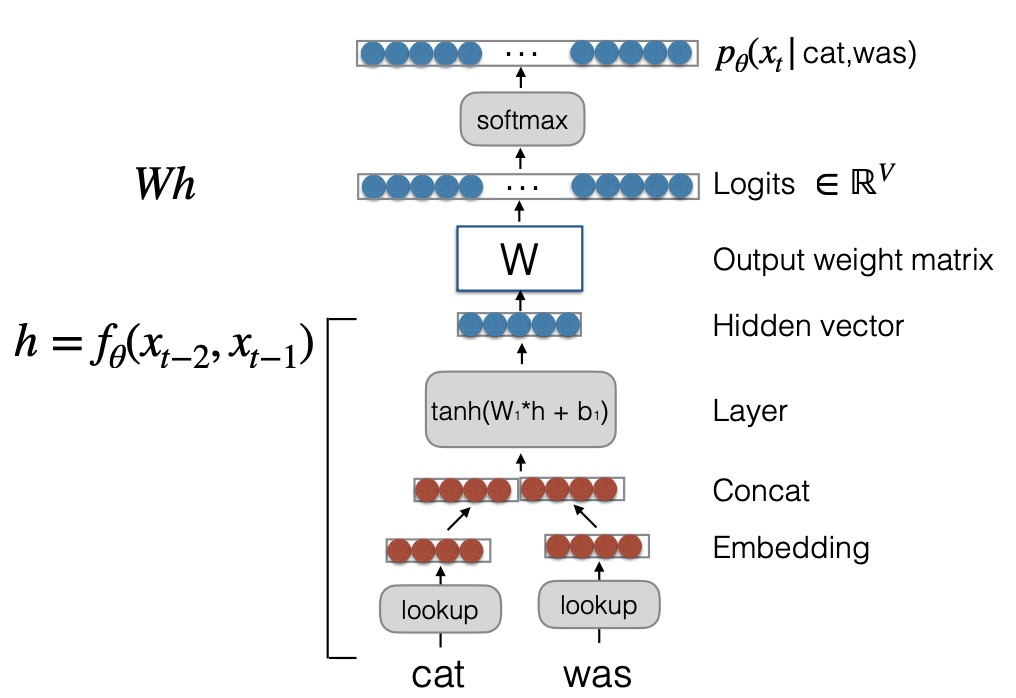
\includegraphics[width=0.5\linewidth]{figs/forward-nn-lm.jpg}
  \caption{An illustration of feedforward neural language 
  model.}
  \label{feedforward-nn-lm}
\end{figure}

Note that since we can make the embeddings of word closed to 
each other if the words have similar meaning, it solves the 
problem of N-gram models that they cannot share strength 
between similar words. Neural models can also condition 
on context with intervening words, which is another advantage
compare to N-gram models.

\subsubsection{Practice tips for neural language models}
It is good to initialize weight matrices
using the \textbf{Xavier initialization} technique, which is 
implmented in function \texttt{nn.init.xavier\_uniform\_} 
in PyTorch. Weight initialization
is important in deep learning models, since it has a huge 
impact on the training results. 
For optimizer, instead of SGD, the most 
standard optimization method is \textbf{Adam}, 
which is also implmented in PyTorch. 
For the choice of learning rate, 
we also have consine learning rate schedule and warmup 
techniques.

Check out paper to learn more about these methods.

\section{Recurrent neural networks}

\subsection{Setup of recurrent neural networks}
A \textbf{sequence model} takes in a sequence $x_1, \dots,
x_T$ and output some hidden state 
\[
f_\theta(x_1, \dots, x_T) \to h_1, \dots, h_T,
\]
where $h_t \in \R^d$. For language modeling, we can have 
\[
p_\theta(\cdot \mid x_{<t}) = \softmax (W h_t^T),
\]
where $W$ is some matrix we learned. 
In contrast, a \textbf{recurrent neural network} (RNN)
has the following recurrence 
\[
h_t = \sigma(W_h h_{t-1} + W_x x_t + b),
\]
where $\sigma$ is some activation function (tanh, ReLU, \dots).
The parameters of the RNN model are $W_h \in \R^{d \times d}$, 
$W_x \in \R^{d \times d}$, and $b \in \R^d$.

RNN can be used for several applications. We can just 
run the RNN on a input sequence and use the final hidden 
state to do sentiment analysis. We can also train 
an output matrix $W$ and use the hidden states to 
produce a sequence.

To train RNNs, we need to construct loss for each 
output (or just the final output if we are doing, 
for example, sentiment analysis) and run the back propogation
algorithm to compute the gradients.

Note that in RNNs, computing $h_t$ requires $h_{t-1}$, 
$h_{t-2}$, \dots, so it is hard to parallelize the training
process. Also, for inference, we generate one token, 
use the new hidden state (newly generated token) for the 
next step, and repeat. We only need to store previous 
hidden state and the computation for a length $T$ sequence
is simply $T$ times the cost of a local computation.

\subsection{Vanishing gradient}

\begin{figure}[h!]
  \centering 
  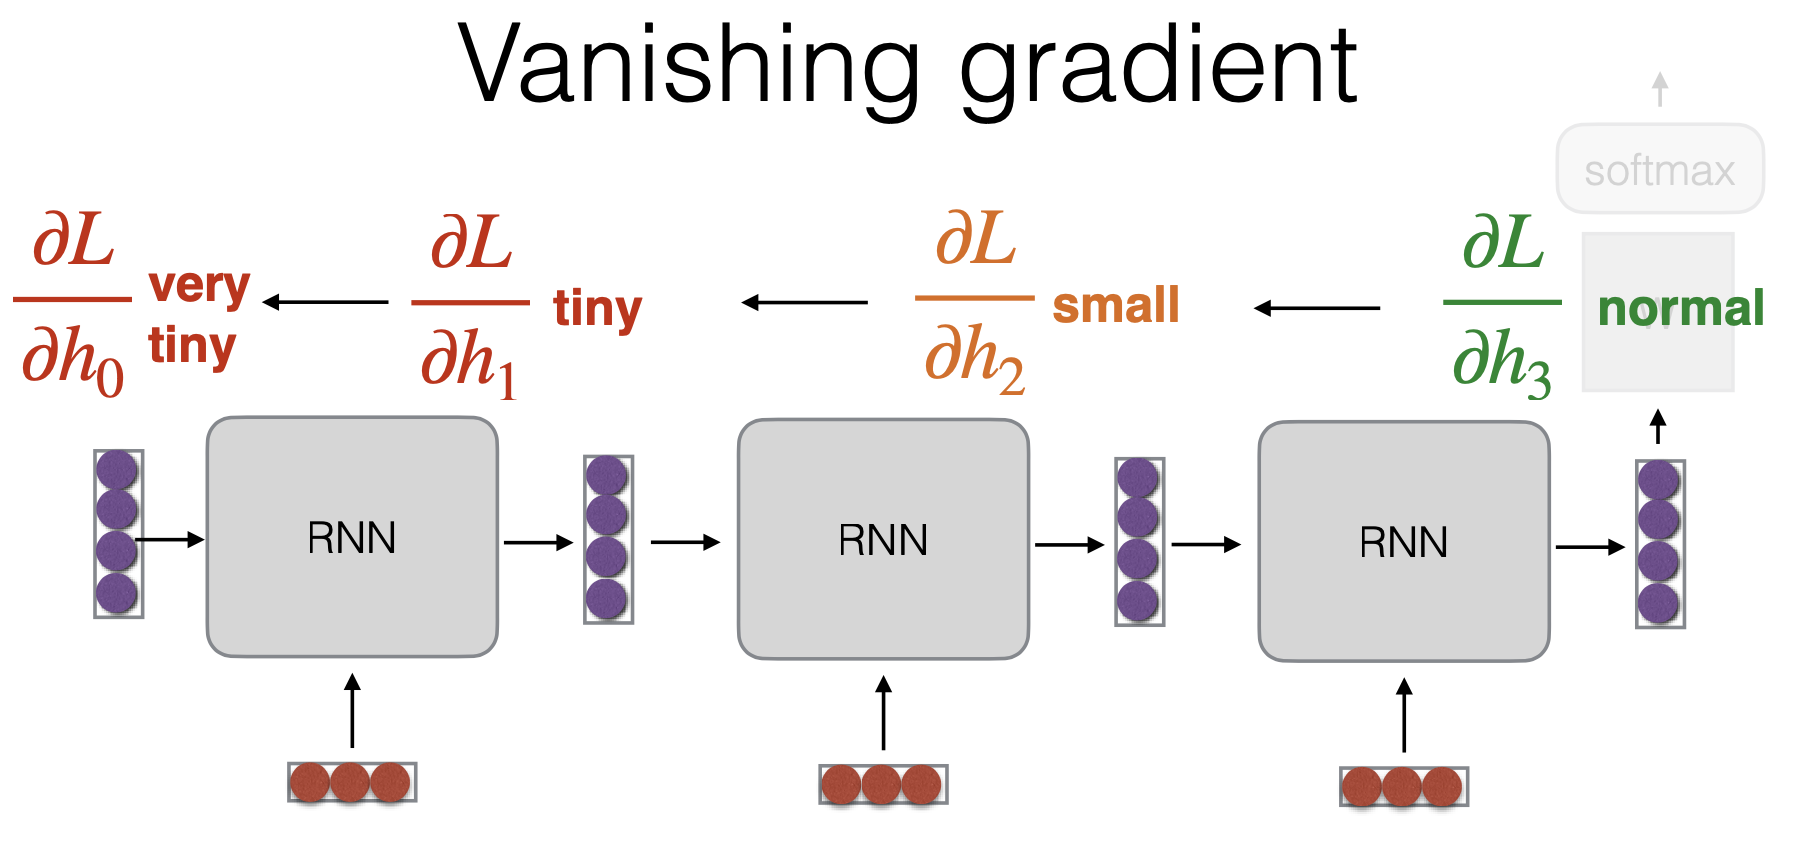
\includegraphics[width=0.5\linewidth]{figs/vanish-grad.png}
  \caption{An illustration of vanishing gradient in RNNs.}
  \label{vanish-grad}
\end{figure}

One problem with RNNs is vanishing gradient, which 
makes the model struggle to learn long-term dependencies.
A illustration of vanishing gradient is in Figure \ref{vanish-grad}.
The mathematical detail can be seen through the following 
equation and derivation. 

*** TO-DO: add math for vanish grad *** 

A solution to this problem is gating and additive 
connections. The basic idea is to 
pass information across timesteps with a learned 
``gate'' $z_t$, and the recurrence would just be 
\[
h_t = (1 - z_t) h_{t-1} + z_t \tilde{h_t}.
\]
More concretely, we replace each RNN black with a Gated 
Recurrent Unit (GRU). 
The GRU has two gates: a ``reset gate'' and an ``update gate''.
The update gate $z_t$ controls how much of the previous 
hidden state should be passed to the current hidden state. 
The reset gate $r_t$ determines how much of the past 
information to forget.
The equations for the GRU are as follows:
\[
\begin{aligned}
z_t &= \sigma(W_z x_t + U_z h_{t-1} + b_z), \\
r_t &= \sigma(W_r x_t + U_r h_{t-1} + b_r), \\
\tilde{h}_t &= \tanh(W_h x_t + r_t \odot (U_h h_{t-1}) + b_h), \\
h_t &= (1 - z_t) \odot h_{t-1} + z_t \odot \tilde{h}_t, \\
\end{aligned}
\]
where in the third equation $\tilde{h_t}$ is a ``candidate state''
and the fourth equation gives recurrent update rule.

A similar but improved architecture compared to GRU 
is Long Short Term Memory (LSTM).

*** TO-DO: add architecture for LSTM ***

\subsection{Encoder-decoder}

The motivation is conditional generation -- generate 
a sequence given a sequence with $p_\theta (y_1, \dots, y_T 
\mid x)$. These models are historically developed for machine 
translation, dialogues, etc.
The architecture of encoder-decoder is 
illustrated in Figure \ref{encode-decode}. The first 
RNN (encoder) read in the sequence $x$ to generate 
the final hidden state (context vector) to represent the whole sequence. 
Then, the second RNN use the context vector to initialize
the inital hidden state and hence generate a new sequence.

\begin{figure}[h!]
  \centering
  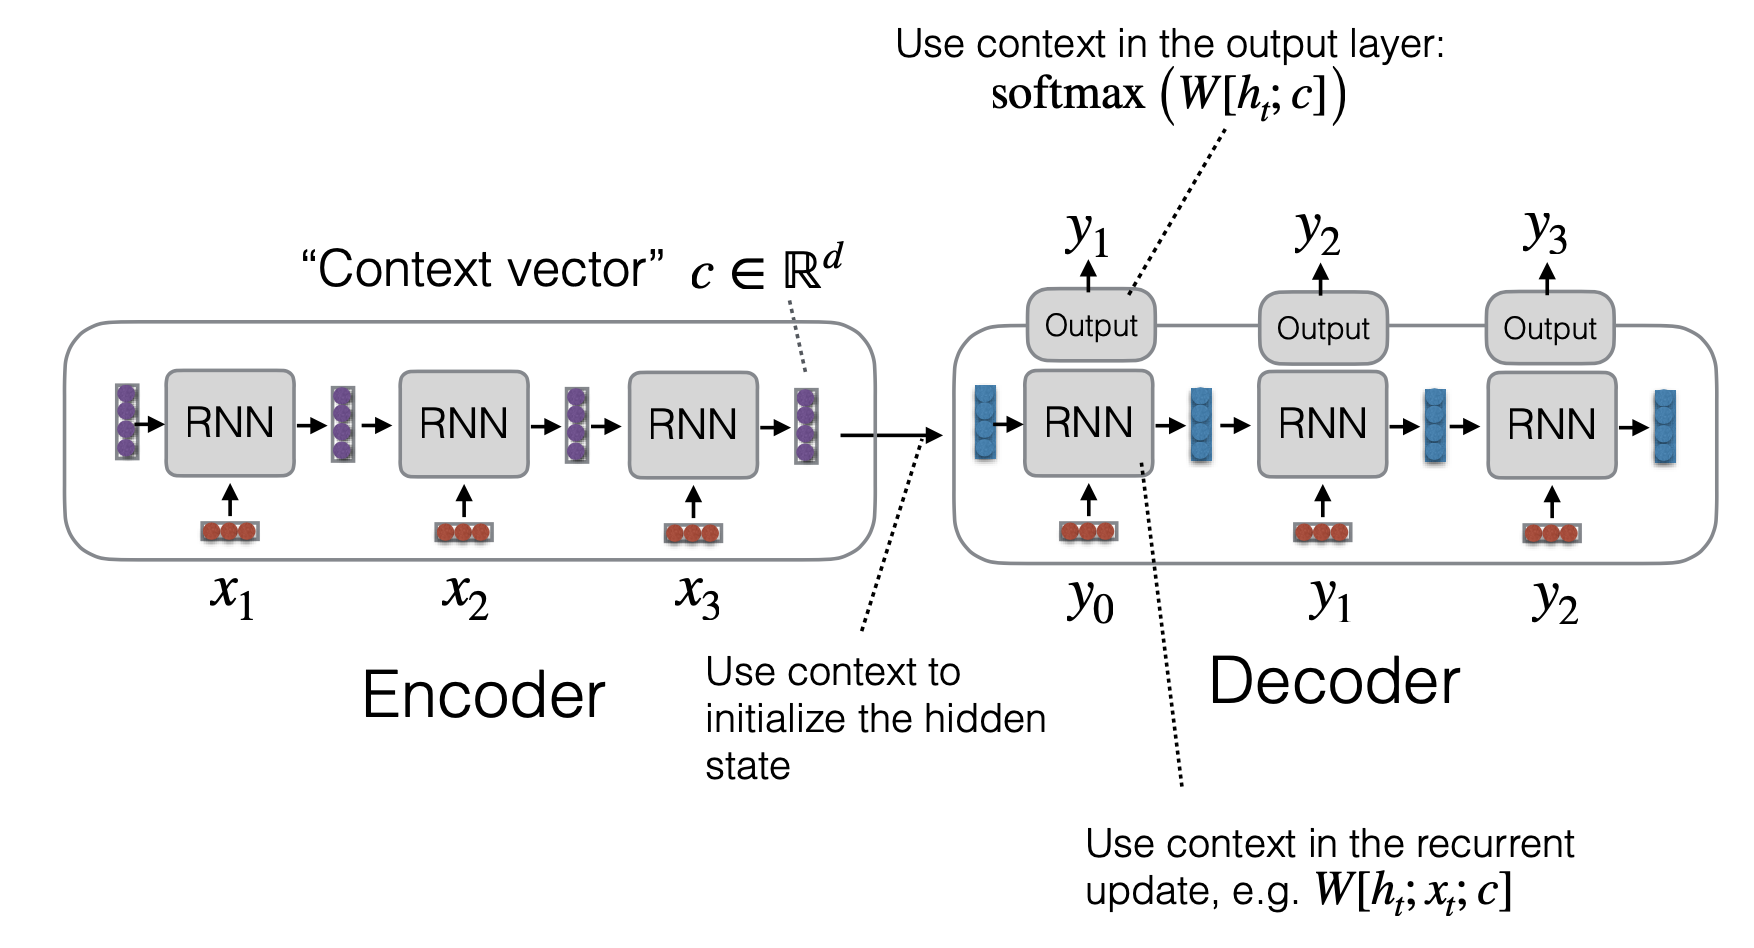
\includegraphics[width=0.6\linewidth]{figs/encode-decode.png}
  \caption{An illustration of encoder-decoder architecture.}
  \label{encode-decode}
\end{figure}

Typically, the parameters of the two RNNs are separator. 
Additionally, having a differentiable connection 
between the two RNNs is important, as the decoder 
need to learn its parameters from the sequence 
generated and the corresponding loss function.

Encoder-decoder only has one context vector for the 
whole sequence. Can we do better?

\subsection{Attention}




\end{document}